\subsection{Mecánica del exoesqueleto} 
    \subsubsection{Diseño mecánico}
        \noindent Considerando la disposición de articulaciones de \cite{hexotrac} presentes en la Figura \ref{fig:EsqArtOri}.
        Se observa que los referenciales no inerciales de las articulaciones $q_{14}$ y  $q_{15}$  están sobrepuestos.
        \begin{figure}[H]
            \centering
            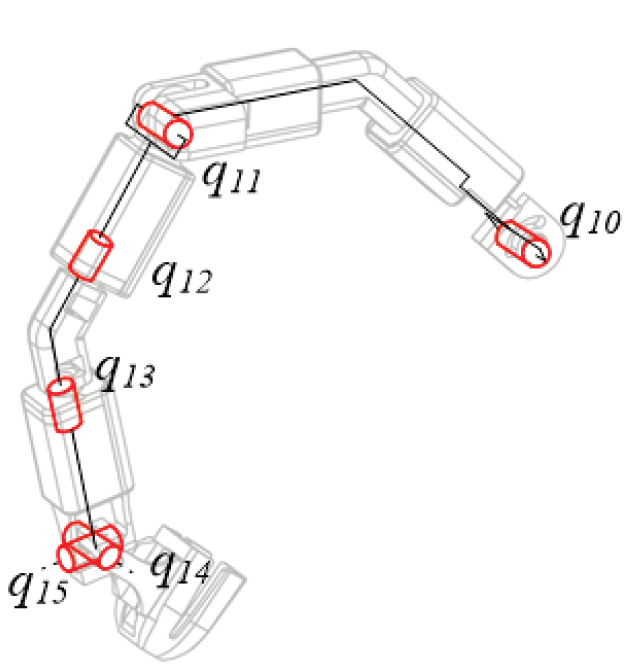
\includegraphics[scale=0.4]{EsquemaArticulaciones.png} 
            \caption{Esquema de las Articulaciones Original}
            \label{fig:EsqArtOri}
        \end{figure}
        Con el fin de facilitar el cálculo recursivo de la cinemática y dinámica del sistema, se optó por agregar un 
        eslabón extra entre ellas, con el fin de conseguir que cada eslabón tenga un referencial asociado.
        Permitiendo así, el diseño del exoesqueleto de 6 GdL expuesto en la Figura \ref{fig:Diseno3D} con una
        posición inicial de \emph{casa} constituido por una cadena cinemática serial abierta de 7 eslabones 
        con articulaciones tipo revoluta. 

        \begin{figure}[H]
            \centering
            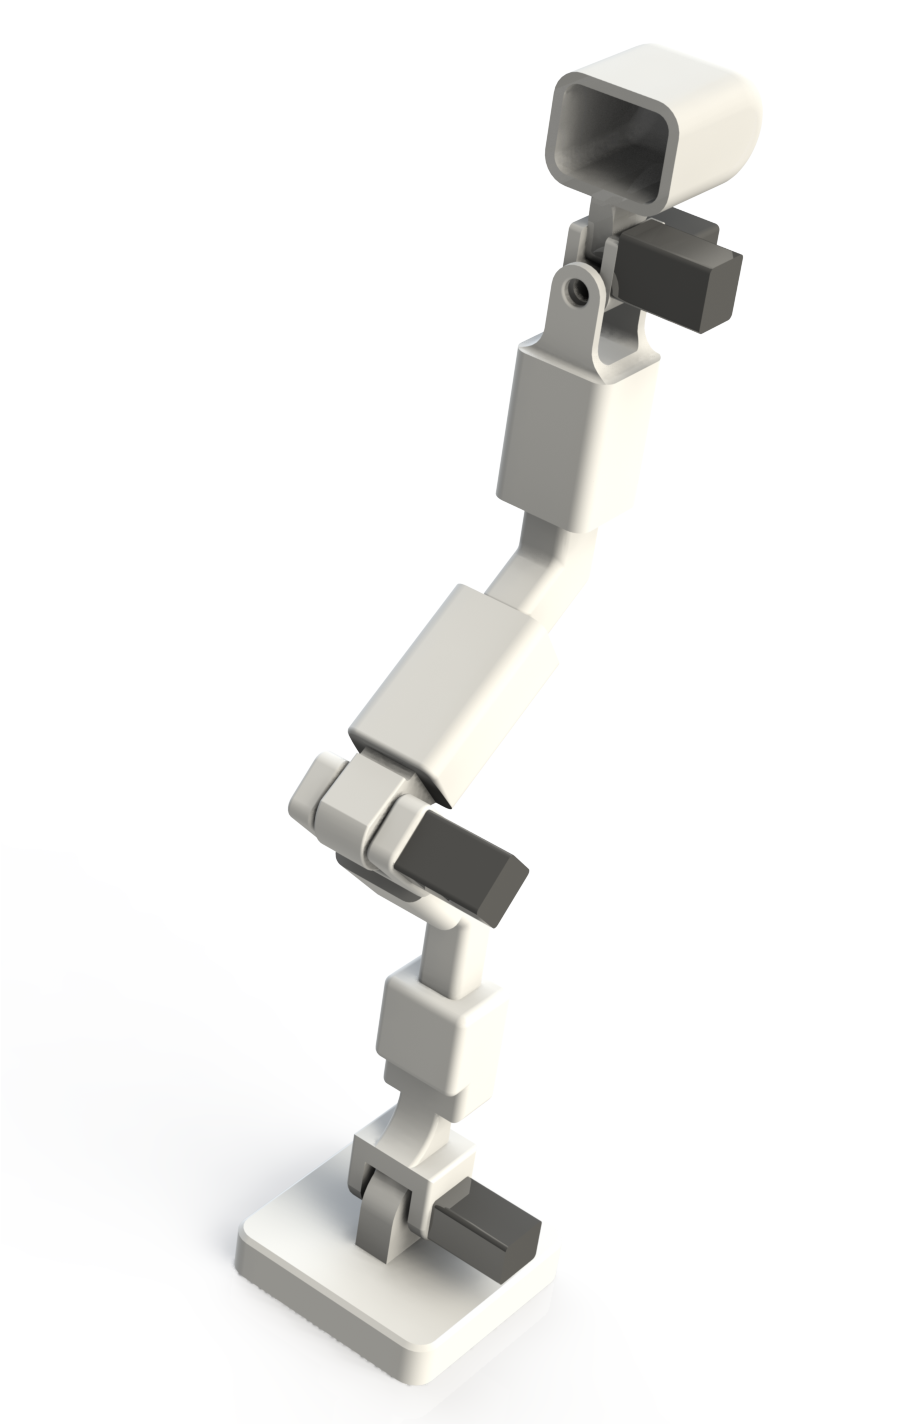
\includegraphics[scale=0.2]{Dedo Vist Isometrica.png} 
            \caption{Diseño 3D}
            \label{fig:Diseno3D}
        \end{figure}

        Donde los eslabones primeros seis eslabones cuentan con el material: \emph{acrilonitrilo butadieno estreno},
        también conocido como \emph{ABS}, polímero termoplástico de utilizado por impresoras 3D. Mientras que para 
        el último eslabón, dedal, se seleccionó \emph{Nylon}, un polímero artificial que 
        pertenece al grupo de las poliamidas. Esto, con el fin de buscar ergonomía y comfort
        ante la interacción con el usuario.

        Respecto a los actuadores, se consideró para cada articulación motores \emph{Pololu -  micro Metal LP} de corriente
        directa con relación de engranes 50:1. Cuenta con dimensiones $24$ x $10$ x $12$ $[mm]$ y masa de $10$ $[g]$.

        Considerando la caracterízación de los eslabones y motores, puede obtenerse los valores de masa y centro de masa
        respecto a su referencial local en las Sección de \ref{tb:masas_cm}, así como el Tensor de Inercia de cada eslabón
        en su centro de masa expuesto en la Sección \ref{Tensores}.


    \subsubsection{Asignación de referenciales}
    \noindent En la Figura \ref{fig:ExoPara} se presenta el modelo acotado de acuerdo al Cuadro
    \ref{tb:dimensiones_referenciales} donde el ángulo $\beta$, equivalente a  $-59.26^\circ $, 
    corresponde al ángulo de azimuth expuesto en el Cuadro \ref{tb:generales_gryma}
    
    \begin{table}[!ht]
        \centering
        \caption{Dimensiones relativas entre referenciales no inerciales}
        \label{tb:dimensiones_referenciales}
        \begin{center}
            \begin{tabular}{ccc}
                Parámetro & [m] \\
                \hline \hline 
                L1 & 0.03235525  \\ 
                L2 & 0.10513390  \\
                L3 & 0.02462267  \\
                L4 & 0.02228474  \\
                L5 & 0.04334075  \\
                L6 & 0.00600000  \\
                L7 & 0.01999013  \\
                L8 & 0.02565247  \\
                L9 & 0.01273194  \\
                L10 & 0.03641522 \\
            \end{tabular}
        \end{center}
    \end{table}

    Además, se aprecia la asignación de referenciales $\Sigma_0$, $\Sigma_1$, $\Sigma_2$,
    $\Sigma_3$, $\Sigma_4$, $\Sigma_5$, $\Sigma_6$ y $\Sigma_7$ de acuerdo a la metodología GRyMA. 
    
    \begin{figure}[H]
        \centering
        \label{fig:referencialesGRyMA}
        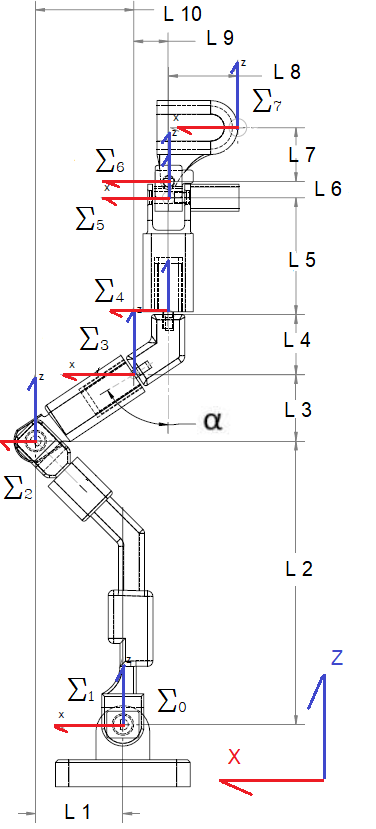
\includegraphics[scale=0.7]{ExoParametrizado.png}
        \caption{Esquema de las Articulaciones Utilizado}
        \label{fig:ExoPara}
    \end{figure}